\documentclass[a4,center,fleqn]{NAR}
\bibliographystyle{NAR-natbib}
\usepackage{color}
\usepackage{xfrac}

\newcommand{\rngcomment}[1]{{\color{red}RNG: #1}}
\newcommand{\bkmcomment}[1]{{\color{blue}BKM: #1}}
\newcommand{\batcave}{BATCAVE }
\newcommand{\beginsupplement}{%
        \clearpage
        \onecolumn
        \setcounter{table}{0}
        \renewcommand{\thetable}{S\arabic{table}}%
        \setcounter{figure}{0}
        \renewcommand{\thefigure}{S\arabic{figure}}%
     }
% Enter dates of publication
\copyrightyear{2008}
\pubdate{31 July 2009}
\pubyear{2009}
\jvolume{37}
\jissue{12}

\articlesubtype{Genomics and Bioinformatics}

\begin{document}

\title{\batcave: Bayesian Analysis Tools for Context-Aware Variant Evaluation}

\author{%
Brian K. Mannakee\,$^{1}$ and
Ryan N. Gutenkunst\,$^{2}$%
\footnote{To whom correspondence should be addressed.
Email: rgutenk@email.arizona.edu}}

\address{%
$^{1}$Mel and Enid Zuckerman College of Public Health, University of Arizona, Tucson AZ
and
$^{2}$Department of Molecular and Cellular Biology, University of Arizona, Tucson AZ}
% Affiliation must include:
% Department name, institution name, full road and district address,
% state, Zip or postal code, country

\history{%
Received January 1, 2009;
Revised February 1, 2009;
Accepted March 1, 2009}

\maketitle

\begin{abstract}
%The accumulation of somatic mutations is an inevitable consequence of tumor development.
Most of the mutations in a tumor at time of diagnosis are present in only a small fraction of all tumor cells.
Identification of these low frequency mutations is increasingly important as evidence has accumulated for their role in treatment resistance, and the value of tumor heterogeneity as a diagnostic biomarker.
The ability to reliably detect low frequency mutations increases as sequencing depth increases, yet false positive identification rates also increase with sequencing depth.
% This dynamic has historically hindered the use of sequencing depths much greater than about 150X average coverage for non-targeted sequencing such as whole exome or whole genome.
Here we present \batcave, an algorithm that uses variant calls produced by MuTect to compute a tumor and site-specific prior probability of mutation for every potential variant, and uses this prior probability to calibrate the posterior probability for every variant.
\batcave uses the mutation profile and allele frequency spectrum of high-confidence mutations to estimate the data generating distribution giving rise to variants.
We show that high-confidence variant calls are sufficient to generate a good estimate of this data generating distribution, and the posterior probabilies of mutation for called variants are better calibrated than those arising from current variant calling algorithms.
The algorithm performs consistently as sequencing depth increases, enabling deeper sequencing and identification of lower frequency variants while providing well calibrated false positive rate expectations.
We provide an R package implementing the \batcave algorithm for use with MuTect output.
\end{abstract}


\section{Introduction}

Cancer develops through the accumulation of somatic mutations and clonal selection of cells with mutations that confer an advantage.
Understanding the evolutionary history of a tumor, including the mutations that drive its growth, the genetic diversity within it, and the accumulation of new mutations, requires accurate variant identification, particularly at low variant allele frequency \cite{Williams2016,Bozic2016,Williams2018,Shi2018}.
Accurate variant calling is also critical for optimizing the treatment of individual patients' disease \citep{Ding2012,Mardis2012,Chen2013,Borad2014,Findlay2016}.
Low frequency mutations challenge current variant calling methods, because their signature in the data is difficult to distinguish from the noise introduced by Next Generation Sequencing (NGS), and this challenge increases with sequencing depth.

Many methods have been developed for calling somatic mutations from NGS data.
The earliest widely used somatic variant callers developed specifically for tumors, MuTect1 and Varscan2, used a combination of heuristic filtering and a model of sequencing errors to identify and score potential variants and set a threshold score designed to balance sensitivity and specificity \citep{Koboldt2012,Cibulskis2013}.
Subsequent research gave rise to a number of alternate strategies, including haplotype-based calling \citep{Garrison2012},
joint genotype analysis (SomaticSniper, JointSNVMix2, Seurat, and CaVEMan,MuClone) \cite{Larson2012,Roth2012a,Christoforides2013,Jones2016,Dorri2019}, allele frequency-based analysis (Strelka, MuTect, LoFreq, EBCall, deepSNV, LoLoPicker, and MuSE) \citep{Saunders2012,Wilm2012,Shiraishi2013b,Gerstung2012,Carrot-Zhang2017,Fan2016}, and ensemble and deep learning methods (MutationSeq, SomaticSeq, SNooPer, and BAYSIC) \rngcomment{Citations?}.
These methods vary in their complexity and specific focus.
But they all implicitly or explicitly assume that the rate of mutation is constant across the genome.

The mutational processes that generate single nucleotide variants in tumors do not act uniformly across the genome.
%Single nucleotide variants arise in tumors at a rate and at genomic locations driven by two main processes. 
The processes of spontaneous mutation that are active in all somatic tissues depend sensitively on local nucleotide context \citep{Nik-Zainal2012a,Alexandrov2015,Lee-Six2018}. 
Additional mutational processes are active in tumors, due to mutagen exposure or defects in DNA maintenance and repair, and these processes are also sensitive to local nucleotide context \citep{Alexandrov2013a,Helleday2014a,Nik-Zainal2016,Kandoth2013,Alexandrov2016}.
The specific mutational processes active in a particular tumor generate its unique mutation profile, and differences within and between tumor types are pronounced \cite{Stephens2005, Burrell2013a, Nakamura2015, Witkiewicz2015, Kumar2016}.
For example, Figure~\ref{NAR-sigfig}, shows mutation profiles from several tumors.
These real tumor mutation profiles show the diversity of profiles seen even within a single cancer.
%Figure \ref{NAR-sigfig} \textbf{a-e} shows several examples of mutation profiles from both real and simulated tumors.

Here we present an enhanced variant-calling algorithm that uses the biology of each individual tumor's mutation profile to improve identification of low allelic frequency mutations.
Our algorithm estimates the tumor's mutation profile using high-confidence variants and then uses that profile as a prior when calling other variants.
Our implementation of the algorithm, \texttt{batcaver}, takes output from the MuTect variant caller as input and returns the posterior probability that a site is variant for every site observed by MuTect.
Using both simulated and real data, we show that the addition of a mutation profile prior to MuTect produces a superior variant caller.
Our algorithm is simple, computationally inexpensive, and can be integrated into numerous other variant callers.
Broad adoption of our approach will enable more confident study of low allelic frequency mutations in tumors in both research and clinical settings.

\begin{figure}
  \begin{center}
  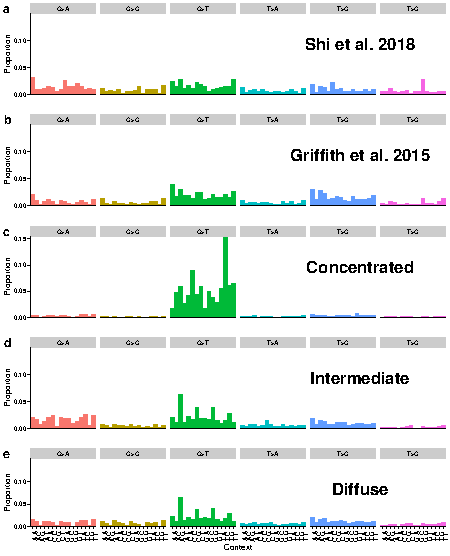
\includegraphics{figures/signatures_only.pdf}
  \end{center}
  \bkmcomment{tumor in F is probably normal breast plus APOBEC. Mention somewhere?}
  \caption{Tumor mutation profiles.
  In each panel, the x-axis corresponds to each of the 96 possible substitution types, and the y-axis is the proportion of total mutations of each type.
  \textbf{(A)} The observed mutation profile of an acute myeloid leukemia used in our real data analysis \cite{Griffith2015}.
  \textbf{(B)} The observed mutation profile of a breast tumor used in our real data analysis \cite{Shi2018}.
  \textbf{(C)}\&\textbf{(D)} The observed mutation profiles of two breast tumors \cite{Alexandrov2019}.
  \textbf{()} A mutation profile used for simulating tumors, made up of equal proportions of COSMIC mutation signatures 1, 7, \& 11.
  \textbf{()} Equal proportions of signatures 1, 4, \& 5.
  \textbf{()} Equal proportions of signatures 1, 3, \& 5.
  \rngcomment{Move simulated profiles to own figure.}
   }
  \label{NAR-sigfig}
 \end{figure}

\section{MATERIALS AND METHODS}
\subsection{Somatic variant calling probability model}

At every site in the genome with non-zero coverage, Next Generation Sequencing produces a vector $\mathbf{x}  = (\{b_i\},\{q_i\}), i = 1\dots \mathrm{d}$ of base calls and their associated quality scores, where $\mathrm{d}$ is local read depth.
Variant callers use the data $\mathbf{x}$ to choose between competing hypotheses:
\begin{equation}
  \label{eqn:hypothesis}
  \begin{array}{l}
    \mathbf{H_0}:\quad \textrm{Alt allele} = m;\quad\nu = 0\\
    \mathbf{H_1}:\quad \textrm{Alt allele} = m;\quad\nu = \hat{f}.
  \end{array}
\end{equation}
Here $m$ is any of the 3 possible alternate non-reference bases and $\nu$ is the variant allele frequency.
The maximum likelihood estimate of $\nu$ is simply $\hat{f}$, the number of variant reads divided by the local read depth.
The posterior probability of a given hypothesis, $\mathrm{P}(m,\nu)$, is the product of the likelihood of the data given that hypothesis and the prior probability of that hypothesis. 
Assuming that reads are independent, this is
\begin{equation}\label{eqn:1}
  \mathrm{P}(m,\nu) = \mathrm{p}(m,\nu) \cdot \prod_{i=1}^{\mathrm{d}} \textrm{f}_{m,\nu}(x_i),
\end{equation}
where $\textrm{f}_{m,\nu}(x_i)$ is the probability model for reads.

Assuming that the identity of the alternate allele and its allele frequency are independent and that $\nu$ is uniformly distributed, Eq.~\ref{eqn:1} becomes
\begin{equation}  \label{eqn:2}
  \mathrm{P}(m,\nu) = \mathrm{p}(m) \cdot \prod_{i=1}^{\mathrm{d}} \textrm{f}_{m,\nu}(x_i).
\end{equation}
The focus of \batcave is to provide a tumor- and site-specific estimate of the prior probability of mutation $\mathrm{p}(m)$.

\subsection{Site-specific prior probability of mutation}
The probability that we have denoted $\mathrm{p}(m)$ in Eq.~\ref{eqn:2} is more precisely the joint probability that a mutation has occurred $M$ and that it was to allele $m$, which we denote $\mathrm{p}(m,M)$.
But $\mathrm{p}(m,M)$ is not uniform across the genome.
Rather it depends on the local genomic context $C$, so its full form is $\mathrm{p}(m,M | C)$ \cite{Buisson2019}.
Assuming that $m$ and $M$ are independent conditional on the genomic context, $\mathrm{p}(m,M \mid C) = \mathrm{p}(m \mid C) \mathrm{p}(M \mid C)$, which we can use Bayes' theorem to further decompose as 
\begin{equation}
  \label{eqn:full_prior}
  \mathrm{p}(m,M \mid C) = \mathrm{p}(m \mid C) \mathrm{p}(C \mid M)\frac{\mathrm{p}(M)}{\mathrm{p}(C)}.
\end{equation}
We next show how to estimate the quantities in Eq.~\ref{eqn:full_prior}.

\subsection{Estimation of the mutation profile}
Many aspects of genomic architecture can affect the somatic mutation rate at multiple scales \cite{Buisson2019}.
Here we focus on a small-scale feature, the tri-nucleotide context, which is known to strongly effect the prior probability of mutation \citep{Nik-Zainal2012a,Alexandrov2015,Lee-Six2018}.
The tri-nucleotide context of a genomic site consists of the identity of the reference base and the 3' and 5' flanking bases.
Folding the central base to the pyrimidines, there are two possible bases at the focal site, and there are four possible bases 3' and 5' of the focal site, yielding $2 \cdot 4 \cdot 4$ possible tri-nucleotide contexts $C$.
At the focal site, a mutation $m$ can be to any of three alternate alleles.
Indexing by the $c=\{1 \dots 32\}$ contexts and by the $m = \{1 \dots 3\}$ alternate bases, we have 96 possible substitution types $S_{m,c}$.
Eq.~\ref{eqn:full_prior} is then
\begin{equation}
  \label{eqn:detailed_prior}
  \begin{array}{rcl}
  \mathrm{p}(\mathrm{S}_{m,c}) &=&  \mathrm{p}(m, M | C = c) \\
                            &=& \mathrm{p}(m \mid C = c) \mathrm{p}(C = c \mid M)\frac{\mathrm{p}(M)}{\mathrm{p}(C = c)}.
  \end{array}
\end{equation}
The first two terms on the right-hand side can be estimated from the observed mutation profile (Figure ~\ref{NAR-sigfig}).
%Here $\mathrm{p}(\mathrm{S}_{m,c})$ represents probability that a substitution of type $\mathrm{S}_{m,c}$ will occur.

We model the observed mutation profile $\mathrm{S}$ (Figure~\ref{NAR-sigfig}\textbf{A}-\textbf{E}) as multinomial with parameter $\boldsymbol{\pi} = \{\pi_{m,c}\}$.
Each element of $\boldsymbol{\pi}$ represents the expected proportion of mutations that are to allele $m$ and in context $c$.
In a tumor with many high-confidence observed mutations, $\boldsymbol{\pi}$ could be estimated directly from the observed mutation profile $S$.
But in practice many entries in $\boldsymbol{\pi}$ would then have zero weight.
We thus model the distribution of $\mathrm{S}$ as Dirichlet-multinomial with pseudo-count hyper-parameter $\boldsymbol{\alpha}$, 
\begin{equation}
\begin{aligned}
  \boldsymbol{\pi} \mid \boldsymbol{\alpha} &\sim \textrm{Dirichlet}(\boldsymbol{\alpha}) \\
  \mathrm{S} \mid \boldsymbol{\pi} & \sim \textrm{Multinomial}(\boldsymbol{\pi}).
\end{aligned}
\end{equation}
In \batcave we use the symmetric non-informative hyper-parameter $\boldsymbol{\alpha} = \boldsymbol{1}$, so a priori mutation is equally likely in any context.

To estimate $\boldsymbol{\pi}$, we identify a subset of high confidence variants, based on an initial calculation of their likelihood given the data.
These are variants for which the evidence in the read data overwhelms any reasonable value of the site-specific prior probability of mutation.
Let $\mathrm{D}$ be the set of high confidence variant calls, which we define as those having posterior odds greater than 10 to 1 without the site-specific prior, and $\mathrm{s} \in \mathrm{D}$ be the substitution type of each mutation in $\mathrm{D}$.
The posterior distribution of $\boldsymbol{\pi}$ is then $\mathrm{p}(\boldsymbol{\pi} \mid \mathrm{D}) \sim \textrm{Dirichlet}(\boldsymbol{\alpha^{\prime}})$ where
\begin{equation}
    \alpha^{\prime}_{m,c} = \alpha_{m,c} + \sum\limits_{\mathrm{s} \in \mathrm{D}} \mathrm{I}\{\mathrm{s} = \mathrm{s}_{m,c}\}.
\end{equation}
Returning to Eq. \ref{eqn:detailed_prior}, given that a mutation has occurred, the posterior probability it occurred in context $c$ is
\begin{equation}
  \label{eqn:post_pred}
  \mathrm{p}(C = c \mid M,\mathrm{D}) = \frac{\sum_{m}\alpha^{\prime}_{m,C = c}}{\sum_{m,c}\alpha^{\prime}_{m,c}}.
\end{equation}
The posterior probability of mutation to allele $m$ given that a mutation has occurred in context $C = c$ is then
\begin{equation}
  \label{eqn:to_allele}
   \mathrm{p}(m \mid C = c,\mathrm{D}) = \frac{\alpha^{\prime}_{m,c}}{\sum_{m} \alpha^{\prime}_{m,C = c}}.
\end{equation}
The prior probability of each particular trinucleotide context $p(C = c)$ is computed simply as the proportion of sequenced trinucleotide contexts that have context $c$.
The R implementation of \batcave ships with pre-computed tables for both whole exomes and whole genomes.

\subsection{Estimation of the mutation rate}
The final piece of Eq. \ref{eqn:detailed_prior} is $p(M)$, the prior probability of mutation, which we specify as the per-base mutation rate $\mu$.
In an exponentially growing and neutrally evolving tumor, branching process calculations \cite{Williams2018} show that the expected total number of mutations $\mathrm{M}$ between two allele frequencies ($f_{min}$,$f_{max}$) is
\begin{equation}
  \label{eqn:mut_rate}
  \mathrm{M}(f_{min},f_{max}) = N\frac{\mu}{\beta}\left(\frac{1}{f_{min}} - \frac{1}{f_{max}}\right).
\end{equation}
The number of bases $N$ is $3\cdot10^9$ for a whole genome and $3\cdot10^7$ for a whole exome.
The quantity $\mu/\beta$ is the effective mutation rate, where $\beta$ is the fraction of cell divisions that lead to two surviving lineages.
We make the simplifying assumption that there is no cell death ($\beta = 1$), so we somewhat over-estimate $\mu$.
We can then estimate $\mu$ by counting observed high-confidence mutations between allele frequencies $f_{min}$ and $f_{max}$.
We can set $f_{max}$ to be the largest allele frequency in $\mathrm{D}$, but we must choose $f_{min}$ conservatively, depending on sequencing depth.
In the R implementation of \batcave, $f_{min}$ is a free parameter.
For this paper, we set $f_{min} = 0.05$, because we are working at high depth.
%A value 0.12 for $f_{min}$ at lower sequencing depth is suggested in Williams et al., 2016~\citep{Williams2016}.
%Equation \ref{eqn:mut_rate} then allows us to estimate $\mathrm{p}(M) = \mu$, and we have a complete tumor-specific specification of the site-specific prior probability of mutation.

\subsection{Likelihood function}
The current implementation of \batcave builds on MuTect, because MuTect reports the log ratio of the likelihood functions for the null and alternative hypotheses (Eq. \ref{eqn:hypothesis}) as \textrm{TLOD} (MuTect1) or \textrm{t\_lod\_fstar} (MuTect2).
We used MuTect 1.1.7 for all analyses in this paper, so we have
\begin{equation}
  \label{eqn:tlod}
    \mathrm{TLOD} = \mathrm{log}_{10}\left(\frac{\prod_{i=1}^{\mathrm{d}} \textrm{f}_{m,\nu = \hat{f}}(x_i)}{\prod_{i=1}^{\mathrm{d}} \textrm{f}_{m,\nu = 0}(x_i)}\right).
\end{equation}
The log posterior odds is the log likelihood ratio (\textrm{TLOD}) plus the log prior odds, so the posterior odds in favor of the alternate hypothesis for a given substitution type is
\begin{equation}
  \label{eqn:computed_posterior}
  \frac{\mathrm{P}(m,\nu = \hat{f})}{1 - \mathrm{P}(m,\nu = \hat{f})} = 10^{\mathrm{TLOD} + \mathrm{logit}_{10}(\mathrm{p}(\mathrm{S}_{m,c}))}.
\end{equation}
Here $\mathrm{p}(\mathrm{S}_{m,c})$ is the prior probability of a substitution of type $\mathrm{S}_{m,c}$, as described in Eq.~\ref{eqn:detailed_prior} and specified in Eq.~\ref{eqn:post_pred}-\ref{eqn:mut_rate}.
When comparing our posterior odds to those of MuTect, we assume a uniform per-base probability of mutation of $3\cdot10^{-6}$ \cite{Cibulskis2013}, so
\begin{equation}  \label{eqn:mutect_posterior}
  \frac{\mathrm{P}_\mathrm{MuTect}(m,\nu = \hat{f})}{1 - \mathrm{P}_\mathrm{MuTect}(m,\nu = \hat{f})} = 10^{\mathrm{TLOD} - 6}.
\end{equation}

\subsection{Implementation}
\rngcomment{Add section about code implementation. What libraries are using, etc.?}

\subsection{Tumor simulations}
We used a neutral branching process with no death and $\mu=3\cdot10^{-6}$ to simulate realistic distributions of allele frequencies.
Tumors were simulated with three different mutation profiles composed of COSMIC mutation signatures (version 2) \cite{XXX}.
\rngcomment{Put COSMIC website as a citation.}
Each simulated profile includes COSMIC signature 1, which is found in nearly all tumors and is associated with spontaneous cytosine deamination.
The ``Concentrated'' profile (Fig.~\ref{XXX}) is an equal combination of COSMIC signatures 1, 7, and 11, which has a large percentage of C $>$ T substitutions such as are often seen in cancers caused by UV exposure.
The ``Intermediate'' profile (Fig.~\ref{XXX}) is an equal combination of COSMIC signatures 1, 4, and 5, which has been associated with tobacco carcinogens and is representative of some lung cancers.
The ``Diffuse'' profile (Fig.~\ref{XXX}) is an equal combination of COSMIC signatures 1, 3, and 5, which has been associated with inactivating germline mutations in the BRCA1/2 genes leading to a deficiency in DNA double strand break repair. \rngcomment{Citations for these signature combinations.}
Simulated variants were sampled from a combination of the Cancer Genome Atlas (TCGA) and Pan-Cancer Analysis of Whole Genomes (PCAWG) databases, which include mutations found in all types of cancer.
Whole genome (100X depth) and whole exome (500X depth) reads were simulated from the GRCh38 reference genome using VarSim \cite{Mu2015} and aligned with BWA \cite{Li2009a}, both with default parameters.
Variants were inserted to create tumors with BAMSurgeon with default parameters~\citep{Ewing2015a} and called with MuTect 1.1.7~\cite{Cibulskis2013} with the following parameters:
\begin{scriptsize}
\begin{verbatim}
java -Xmx24g -jar $MUTECT_JAR --analysis_type MuTect \
        --reference_sequence $ref_path \
        --dbsnp $db_snp \
        --enable_extended_output \
        --fraction_contamination 0.00 \
        --tumor_f_pretest 0.00 \
        --initial_tumor_lod -10.00 \
        --required_maximum_alt_allele_mapping_quality_score 1 \
        --input_file:normal $tmp_normal \
        --input_file:tumor $tmp_tumor \
        --out $out_path/$chr.txt \
        --coverage_file $out_path/$chr.cov
\end{verbatim}
\end{scriptsize}
Variants identified by MuTect are labelled as to whether they pass all filters, fail to pass only the the evidence threshold \textrm{tlod\_f\_star} filter, or fail to pass any other filter. 
Variants that passed all filters or failed only \textrm{tlod\_f\_star} were then passed to \batcave for prior estimation and rescoring.

\subsection{Real data}
We analyzed two real data sets, one from an acute myeloid leukemia (AML)~\cite{Griffith2015} and one from a multi-region sequencing experiment in breast cancer~\cite{Shi2018}.
We downloaded the normal and primary whole-genome AML tumor bam files from dbGaP accession number phs000159.v8.p4.
Griffith et al.\ generated a platinum set of variant calls for this tumor~\cite{Griffith2015}, which we used for our true positive dataset.
We downloaded the normal and tumor whole-exome breast cancer bam files from NCBI Sequence Read Archive accession SRP070662.
Shi et al.\ generated a gold set of variant calls for each tumor region sequenced~\cite{Shi2018}, which we used for our true positive dataset.
We called variants using Mutect 1.1.7 as in our simulations, except that both these data sets were originally aligned to GRCr37, so we used that reference.
\rngcomment{Did MuTect fail to call anything we know is there?}

\subsection{Calibration metric}
The quantify the difference in calibration between MuTect and \batcave, we use the Integrated Calibration Index \cite{Austin2019}.
Briefly, a loess-smoothed regression was fit by regressing the binary (True=1,False=0) true variant classification against the reported posterior probability for both MuTect and \batcave.
For a perfectly calibrated caller, the regression fit would be the diagonal line $y=x$, and the Integrated Calibration Index is the average distance between the fit and that line.


\section{RESULTS}
We implemented \batcave as a post-call variant evaluation algorithm to be used with MuTect (Versions 1.1.7 or $>$2.0) \cite{Cibulskis2013}.
\batcave extracts the log-likelihood ratio for each potential variant site from the MuTect output, and then it uses that ratio to separate the potential sites in to high- and low-confidence groups.
The mutation profile is estimated from the high confidence sites, and the posterior probability of mutation is then recomputed for all sites.
The \batcave algorithm is inexpensive, processing 22,000 variants per second on a typical desktop computer, which corresponds to roughly 100 seconds to process a 500x exome and 2,000 seconds for a 100x whole genome.

To test the performance of \batcave, we generated six different tumor/normal pairs, corresponding to 100x whole genomes and 500x whole exomes for three different mutation profiles.
The three mutation profiles were chosen to resemble a melanoma (concentrated), a lung cancer (intermediate), and a BRCA-driven breast cancer (diffuse) (Fig.~\ref{XXX}\textbf{A-C}).
We also tested \batcave using two real cancer data sets, a whole-genome Acute Myeloid Leukemia (AML) \cite{Griffiths2015} and a whole-exome multi-region breast cancer \cite{Shi2018}.
In both, deep sequencing and variant validation were performed with the specific purpose of evaluating tumor variant calling pipelines.

\begin{figure}
  \begin{center}
  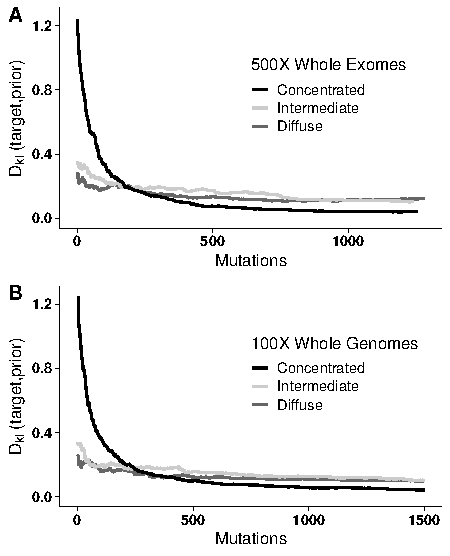
\includegraphics{figures/kl_only.pdf}
  \end{center}
  \caption{Convergence of the site-specific prior to the data generating distribution. Plotted is the Kullback-Leibler divergence between the estimated and simulated profiles versus number of incorporated mutations, for \textbf{(A)} whole exomes and \textbf{(B)} whole genomes.
  \rngcomment{Zoom panel B into relevant region of plot ($\sim$1000 mutations). What is notation (target || prior)?}}
\label{NAR-kl_fig}
\end{figure}

\subsection{Convergence of the prior}
To improve performance, the context-dependent prior probability of mutation must converge to a good representation of the data generating distribution within the set of high-confidence mutations.
When applied to simulated whole exome and whole genome data, the prior converges within a few hundred mutations (Fig.~\ref{NAR-kl_fig}).
For comparison, in our simulated data sets the number of high-confidence mutations ranges between 1500 and 5000, and for a real acute myeloid leukemia it is over 17,000~\cite{Griffith2015}.

%We use the Kullback-Leibler (KL) divergence as a measure of the distance (or entropy difference) between the estimated prior and the actual simulated data generating distribution.
%In Figure~\ref{NAR-kl_fig} we order mutations by descending MuTect probability value, and compute the KL divergence between the prior after adding each mutation and the data generating distribution.
%For both whole exome and whole genome the prior converges to the data generating distribution easily within the number of available high-confidence mutations, which for the leukemia~\citep{Griffith2015} is over 17000, and for our simulated data sets ranges between 1500 and 5000.

  \begin{figure*}
    \begin{center}
    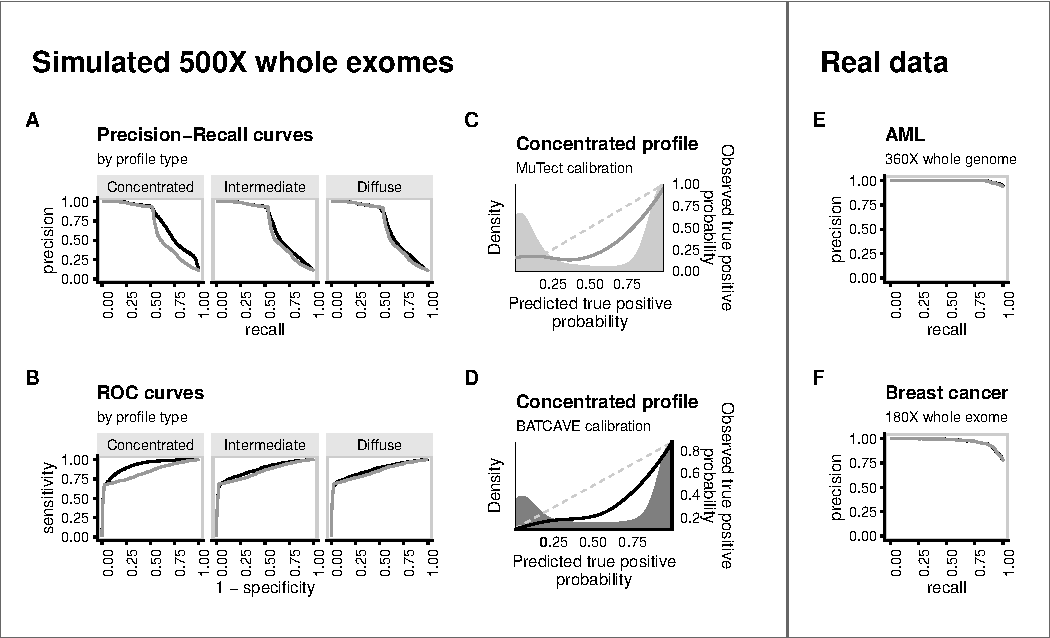
\includegraphics{figures/fig_wes.pdf}
    \end{center}
    \caption{Variant-calling performance on both simulated and real data.
    \textbf{(A)} Precision-recall curves and \textbf{(B)} receiver operating characteristic curves for different mutation signatures.
    \rngcomment{Make labels for \batcave and MuTect in A much bigger. Add similar labels to B.}
    \rngcomment{Move "Synthetic 500x whole exomes" to above A\&C. Add similar label for B\&D}
    \textbf{(C)} and \textbf{(D)} Shaded regions show distributions of posterior probabilities for tree positive variants, and the smooth line shows the loess-smoothed relationship, from which the Integrated Calibration Index is calculated. For a perfectly calibrated caller, that curve would match the dashed y=x line. 
    \rngcomment{Remove dark edges of distributions. Make diagonal line dashed.}
    \textbf{(E)} and \textbf{(F)} Precision-recall curves for real data in which substantial validation was performed
    \rngcomment{Label plots with what type of cancer they are, plus depth.}.}
  \label{NAR-wes_fig}
  \end{figure*}
  
  
\begin{table*}[b]
  \tableparts{%
  \caption{Performance characteristics as measured for all data sets.}
  \label{table:01}%
  }{%
  \begin{tabular*}{\textwidth}{@{}lllllllll@{}}
  \toprule
  Depth & Mutation profile & $\mu$ & AUROC & & AUPRC & & ICI & 
  \\
  & & (estimated) & MuTect & \batcave & MuTect & \batcave & MuTect & \batcave
  \\
  \colrule
  100X whole genome & Concentrated & 3.6e-7 & .987 & .993 & .972 & .975 & .117 & .287
  \\
  100X whole genome & Intermediate & 3.2e-7 & .987 & .989 & .972 & .973 & .118 & .214
  \\
  100X whole genome & Diffuse & 3.2e-7 & .988 & .989 & .971 & .973 & .120 & .219
  \\
  500X whole exome & Concentrated & 3.6e-7 & .848 & .929 & .674 & .758 & .138 & .109
  \\
  500X whole exome & Intermediate & 3.6e-7 & .847 & .881 & .677 & .706 & .108 & .112 
  \\
  500X whole exome & Diffuse & 3.6e-7 & .850 & .873 & .676 & .698 & .105 & .116
  \\
  real AML \cite{Griffith2015} & Actual & 3.6e-8 & -- & -- & .995 & .996 & -- & --
  \\
  real breast \cite{Shi2018} & Actual & 3.6e-8 & -- & -- & .972 & .972 & -- & --
  \\
  \botrule
  \end{tabular*}%
  }
  {$\mu$ = per-base mutation rate, AUROC/AUPRC = area under ROC/PRC curve, ICI = Integrated calibration index.}
 \end{table*}

\subsection{Tests using simulated data}
We assessed classification performance using the areas under both the receiver operating characteristic and the precision-recall curves, because the classes are unbalanced (approximately 5 to 1 ratio of false to true variants in our simulated data).
By both metrics \batcave outperforms MuTect (Fig.~\ref{NAR-wes_fig}\textbf{A}\&\textbf{B} and Table~\ref{table:01}).
The extent of the performance difference is dependent on both the sequencing depth and the concentration of the mutation signature.
Deeper sequencing and more concentrated mutation signatures increase the performance advantage of \batcave. 

For all simulated tumors, the estimated mutation rate is approximately $3\cdot10^{-7}$ (Table~\ref{table:01}), which is lower than the simulated rate of $3\cdot10^{-6}$.
This is due to restrictions with BAMSurgeon, such as sequencing depth and quality, that prevent 100\% of simulated variants from being inserted into the reads.

We also assessed the calibration of \batcave, assessing the likelihood that a potential variant with a given posterior probability is actually a true variant.
We measured overall calibration performance using the Integrated Calibration Index (ICI) \cite{Austin2019}, which measures the difference between predicted and observed probabilities, weighted by the density of the predicted probabilities.
This metric is particularly useful in our case, because the density of posterior probabilities is bi-modal (Fig.~\ref{NAR-wes_fig}C\&D).
A large fraction of true negative variants have posterior probabilities less than $10^{-4}$, far below any meaningful threshold, so we evaluate calibration only on potential variants with posterior probability greater than 0.01.
For these potential variants, \batcave tends to increase posterior probabilities of low probability but true variants (density curves in Fig.~\ref{NAR-wes_fig}C\&D) while decreasing probabilities of low probability but false variants.
For 500X tumors, the calibration of \batcave is better than MuTect across the full spectrum of posterior probabilities, while for 100X whole genomes the calibration is slightly worse (Figure \ref{NAR-wgs_fig} and Table \ref{table:01}).
This is because that there are few low probability true positive variants in tumors sequenced to 100X depth.
As with the other metrics, the advantage of \batcave increases with the concentration of the mutation profile the sequencing depth.

\begin{figure}
  \begin{center}
  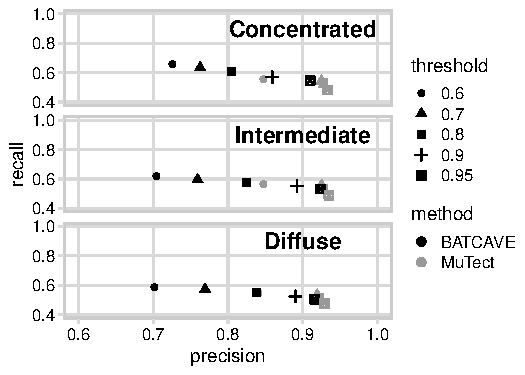
\includegraphics{figures/ppv_wes.pdf}
  \end{center}
  \caption{Calibration of posterior probability. 
  For realistic thresholds, posterior probabilities are more accurately calibrated for \batcave than MuTect, no matter how concentration the mutation profile is.}
\label{NAR-ppv_fig}
\end{figure}

In practice, accurate calibration is most important for variants with high posterior probability.
For variants with posterior probability between 60 and 90\%, \batcave is substantially better calibrated than MuTect (Fig.~\ref{NAR-ppv_fig}\&\ref{NAR-ppv_wgs_fig}).
For any posterior probability above 70\%, MuTect has a false positive rate of roughly 8\%, whereas \batcave has a false positive rate that decreases as posterior probability increases.
The cost of MuTect's compression is recall, which is 3-5\% worse than \batcave at 95\% posterior probability, and 3-7\% worse at 90\%, depending on mutation profile concentration.
At any posterior probability \batcave returns a larger fraction of all positive calls than MuTect.
%Figure~\ref{NAR-ppv_wgs_fig} shows results for 100X whole genomes, where the results are similar for precision.

\subsection{Tests using real tumor data}
We tested \batcave using two data sets for which deep sequencing and variant validation were performed with the specific purpose of evaluating tumor variant calling pipelines.
We considered only precision-recall comparisons for these data, because the validation procedure yields true positives but not comprehensive true negatives. \rngcomment{Is  a correct statement?}

Griffith et al.\ sequenced the whole genome of an acute myeloid leukemia (AML) primary tumor to a depth of $>$360X and used targeted sequencing to validate nearly 200,000 mutations~\cite{Griffith2015}.
We estimated a per-base mutation rate for this tumor of $4\cdot10^{-8}$, which would be considered normal in AML. \rngcomment{Really need a citation for this!}
For both MuTect and \batcave, the precision-recall curve is almost perfect for the validated variants (.995 \& .996 area under the curve) (Fig.~\ref{NAR-wes_fig}E and Table~\ref{table:01}).

Shi et al.\ performed multi-region whole exome sequencing on 6 individual breast tumors to a mean target sequencing depth of $160\mathrm{X}$ and validated all variants identified by three different variant calling pipelines~\cite{Shi2018}.
%We downloaded aligned reads for this tumor, and called variants with MuTect 1.1.7 as described in Materials \& Methods.
We estimated a per-base mutation rate for this tumor of $4\cdot10^{-8}$. \rngcomment{Any comment on this result?}
and the area under the precision-recall curve is identical (.972) for MuTect and \batcave (Figure~\ref{NAR-wes_fig}\textbf{F} and Table \ref{table:01}).
For the validated variants, MuTect and \batcave yield almost identical precision-recall curves (Fig.~\ref{NAR-wes_fig}F and Table~\ref{table:01})




\section{DISCUSSION}
 
\rngcomment{I worry that this bit about very high depth sequencing is going to be problematic in review, because it's not a problem we're solving. We're helping, but not making huge changes.}
%Deep sequencing is necessary to measure intra-tumor heterogeneity \citep{Shi2018}, identify subclonal driver and resistance alleles \cite{Griffith2015}, and probe the mutational landscape of cancer in general \cite{Zehir2017}.  
%Current approaches to very high depth next-generation sequencing \cite{Griffith2015}, however, require combining calls from multiple variant calling algorithms and then validating these calls via ultra-deep sequencing.
%We believe that much of the need for multiple variant callers could be alleviated by improvements to the statistical model used to evaluate the evidence presented by the sequenced reads. 

\batcave is an algorithm that leverages the biology of individual tumor mutation profiles to improve identification of low allelic frequency somatic variants.
Our current implementation is built on MuTect, one of the most widely used somatic variant callers.
\batcave improves on the classification accuracy of MuTect in synthetic data (Fig.~\ref{NAR-wes_fig}A-D and Table~\ref{table:01}) across the entire range of recall and specificity.
Moreover, \batcave is better calibrated than MuTect at relevant posterior probability thresholds (\ref{NAR-ppv_fig}), allowing researchers and clinicians to make informed choices about the trade-off between precision and recall.
For real data, testing on validated calls shows that \batcave does not degrade performance for variants that are relatively easy to identify (Fig.~\ref{NAR-wes_fig}E\&F).
The \batcave algorithm can thus be included in a wide variety of sequencing pipelines.

The \batcave algorithm incorporates genomic context into the probabilistic model for variant calling.
Our current implementation focuses on trinucleotide context, which is known to have a large effect on local mutation rates \cite{Martincorena2015,Hollstein2017}.
There are, however, many other aspects of genomic context that can affect local mutation rates, including replication timing, expression level, and chromatin organization \cite{Buisson2019,Schuster-Bockler2012,Pleasance2010}. 
\rngcomment{Move individual citations to the factors they support.}
These additional forms of context could also be incorporated into the \batcave mutation prior.
In fact, they may be simpler to incorporate than trinucleotide context, because their effect on the prior may vary less among tumors. \rngcomment{Can we back this assertion up?} 
In the long run, we believe that incorporating more tumor biology into variant calling models will often lead to improved performance.

\rngcomment{Got here...}

\batcave resembles an empirical Bayes approach, but is not really empirical Bayes.
In fact, variants are best described as sequential samples from a data generating distribution represented by the mutation profile.
Early mutations are classified with low error, while later mutations are classified with less certainty.
We show here that sequential updating of the dirichlet-multinomial posterior converges to the true data generating distribution using the set of early mutations.
Along with the assumption that tumor evolution is approximately neutral, this allows us to generate a tumor and site-specific prior that sharpens the classification and calibration of later mutations.
Thus, \batcave is best described as an algorithm trained on early mutations.

\bkmcomment{this needs more work}
We simulate tumors with three mutation profiles, and evaluate two real tumor data sets.
Among these performance is best with the most concentrated simulatin profile.
The intermediate and diffuse mutation profiles are designed to represent baseline or minimal profiles of Lung and Breast tumors respectively.
In fact, lung and breast tumors have heterogeneous mutation profiles with a wide range of levels of concentration.
The Acute Myeloid Leukemia we evaluated has a particularly diffuse profile, which is common for these tumors \cite{Alexandrov2019}.


These mutations are in some sense \textit{easy} to call, since at least one variant caller did in fact call them.
At the same time, there is no way to compute true and false negative fractions for these data sets.
As such, it is not surprising that the performance of MuTect and \batcave are similar because the universe of variants under consideration in these experiments are by definition "callable" by at least one variant detection pipeline, and MuTect is among the most sensitive and specific variant callers \cite{Griffith2015,Cibulskis2013}.
%We are unable to study calibration in real data, because complete false positive/true negative data for real data is not available. 
%Deep sequencing experiments where a large random sample of uncalled potential variants, as well as a random sample of variant with no reads at all present, would give much-needed insight into the differences in statistical models in variant calling.


We have chosen to implement \batcave as a post-calling algorithm for exclusive use with MuTect because MuTect presents a simple model and a well-tested set of heuristic filters.
MuTect is widely used, has state of the art sensitivity and specificity, and includes numerous heuristic filters and alignment adjustments that reduce the prevalence of sequencing errors in results \cite{Griffith2015}.
However, the model is very general, and in principle there is no barrier to using the method with other variant callers.
For instance Strelka2, another widely used variant caller, computes a joint posterior probability over tumor and normal genotypes where the prior probability that the tumor carries a somatic mutation at a given site is set to a constant \cite{Kim2018}.
Modifying the algorithm to work with the Strelka statistical model would involve replacing the constant prior with a tumor and site-specific prior for each potential variant, exactly as we have done with MuTect.

The R implementation \texttt{batcaver} adds 1 second per 22,000 variants evaluated to a standard GATK best practices variant calling pipeline. 
The majority of the computational overhead in \batcave is associated with extracting the tri-nucleotide context for each potential variant site from the reference genome.
Since most variant callers are already walking the reference genome as part of the calling process, extracting the tri-nucleotide context simultaneously would dramatically reduce the computational overhead associated with implementing \batcave.

We hope that the availability of this algorithm will have a positive effect on the cost/benefit ratio of deeper sequencing in both research and clinical applications.
One size does not fit all with respect to the evidence threshold. 
Users are interested in true and false positive fractions, and users of different types will have different trade-offs in terms of precision and recall.
We present \batcave, and the R package \texttt{batcaver} to provide the user with a more accurate sense of these trade-offs.

% \section{CONCLUSION}
% \bkmcomment{I looked at a bunch of NAR methods papers, and none include a conclusions section, so I moved it to the last paragraph of discussion.}

\section{Software Availability}
\bkmcomment{working on this today}

github for source code

zenodo for figures, simulations

zenodo for package at time of bioarxiv

\section{Data Availability}
COSMIC mutation signatures version 2 is available at \footnotesize{https://cancer.sanger.ac.uk/cosmic/signatures\_v2}.



\section{ACKNOWLEDGEMENTS}

This work was supported by the National Science Foundation via Graduate Research Fellowship award number DGE-1143953 to BKM and by the National Institute of General Medical Sciences of the National Institutes of Health under award number R01GM127348 to RNG.
We thank Prof.\ Edward J. Bedrick for fruitful discussions about the statistical model.

\subsubsection{Conflict of interest statement.} None declared.

\bibliography{caller_paper}

\beginsupplement
\section{Supplememtary Figures}

\begin{figure}[b]
  \begin{center}
  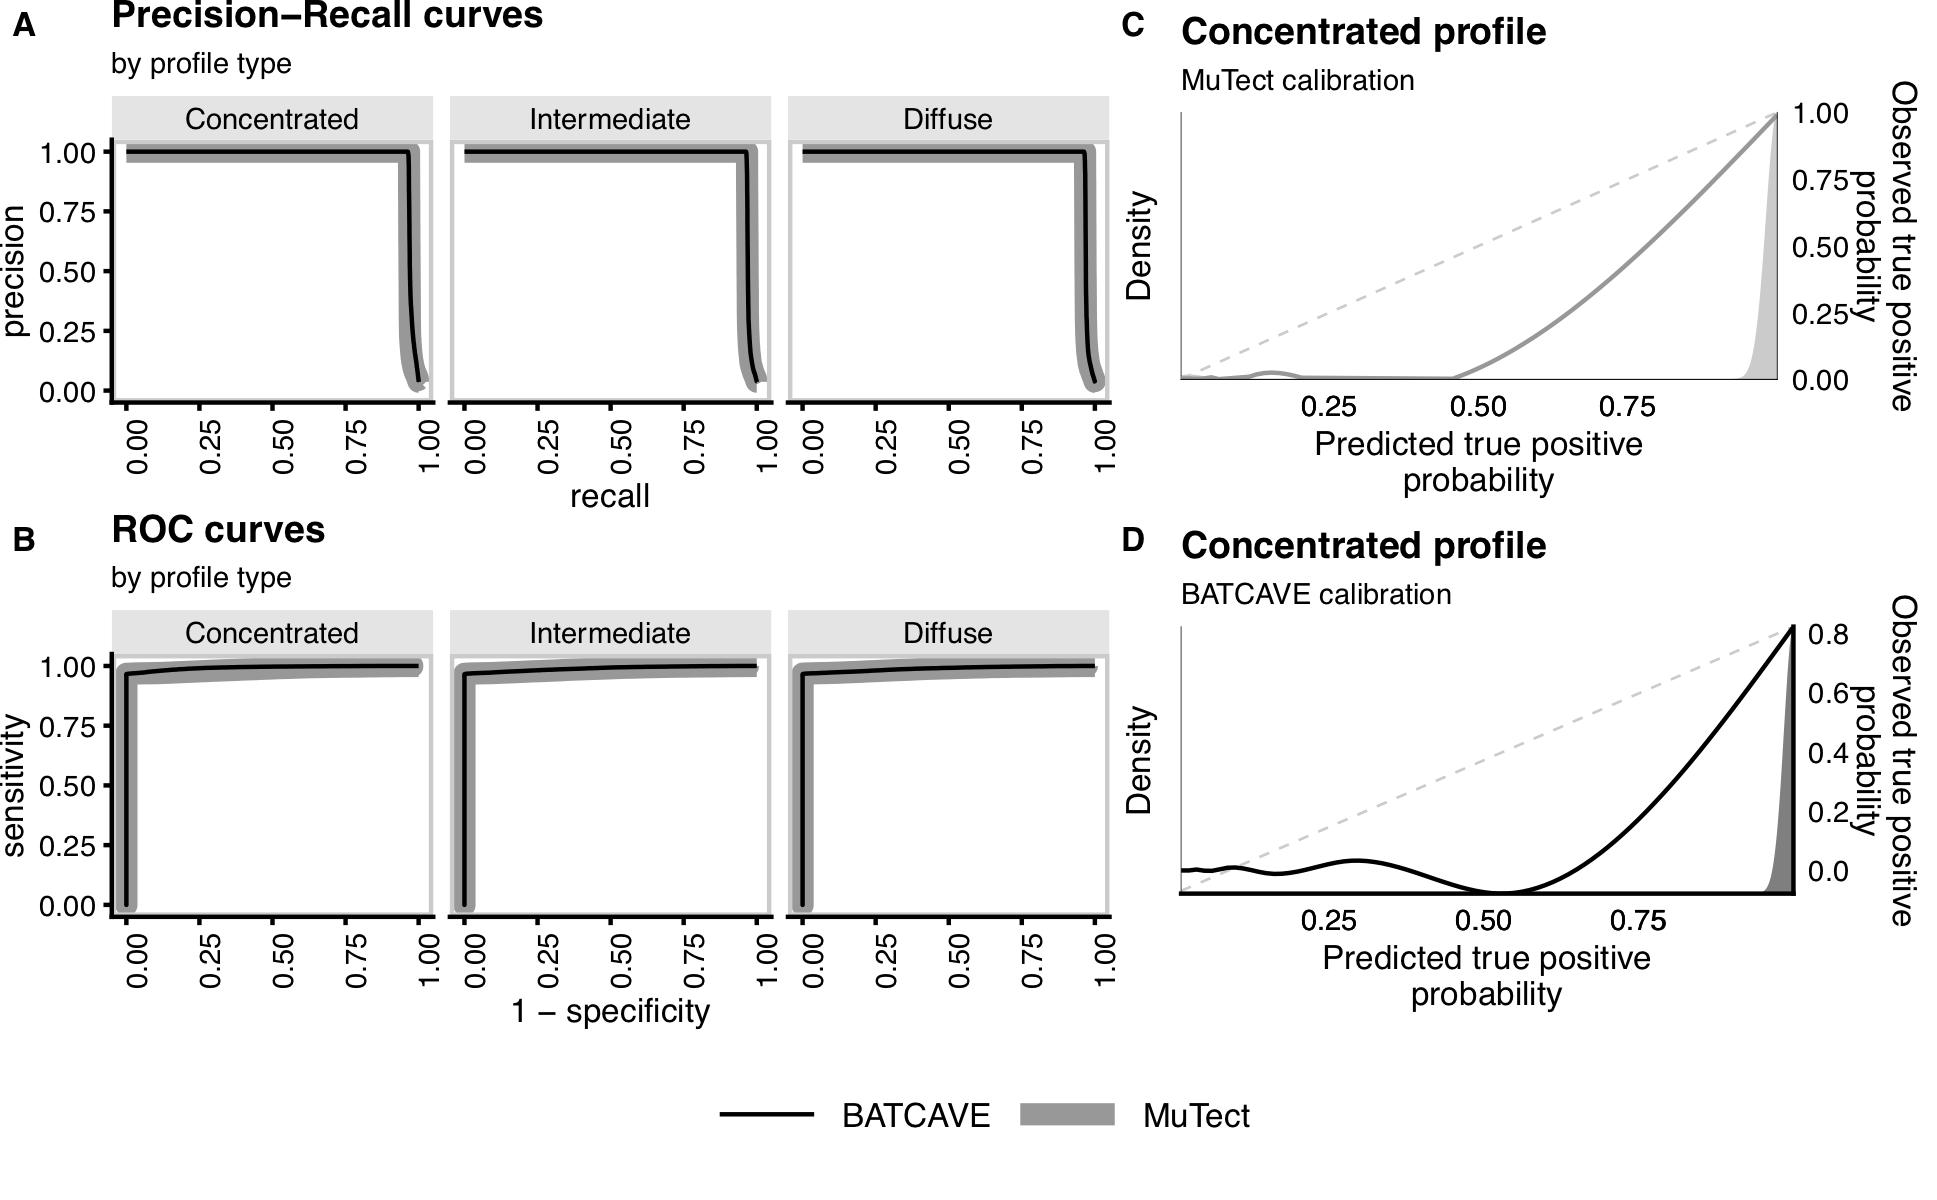
\includegraphics[width=\textwidth]{figures/fig_wgs.png}
  \end{center}
  \caption{Model performance on 100X simulated whole genome.
  \textbf{(A)} Precision recall curves and \textbf{(B)} Reciever operating characteristic curves for 3 mutation signatures.
  Distribution of estimated true positive probabilities for true positive  variants for \textbf{(C)} the MuTect model and \textbf{(D))} the \batcave model.
  A perfectly calibrated model would generate the diagonal line.}
\label{NAR-wgs_fig}
\end{figure}



\clearpage
\begin{figure}
  \begin{center}
  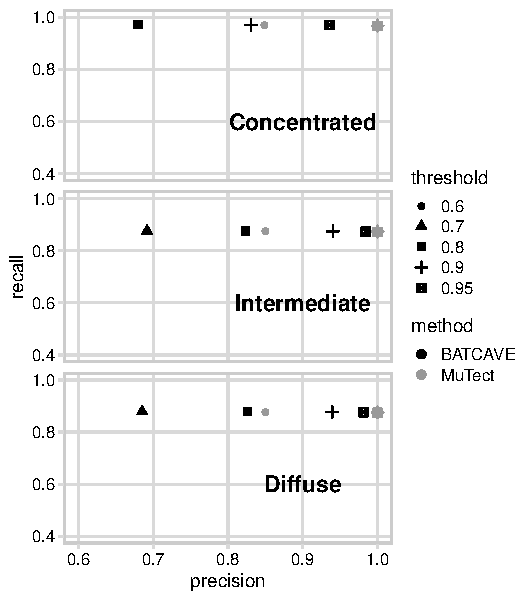
\includegraphics{figures/ppv_wgs.pdf}
  \end{center}
  \caption{Model performance on 100X simulated whole genome. 
  Positive predictive values vs. Recall for five different probability cutoffs. 
  Note the restricted axes to improve readability of points.}
\label{NAR-ppv_wgs_fig}
\end{figure}

\end{document}

